\documentclass{these}

\newcommand{\diagscale}[2]{%
\begin{minipage}[c]{#1}
\includegraphics[width=#1]{#2}
\end{minipage}}

\newcommand{\diagscaleb}[2]{%
%\begin{minipage}{#1}
\includegraphics[width=#1,origin=B]{#2}
%\end{minipage}
}

\begin{document}

\[
\diagscale{1.2cm}{g} = \diagscale{1.2cm}{g0} + \diagscale{1.2cm}{g0}
\diagscale{1.2cm}{Sigma} \diagscale{1.2cm}{g} = \diagscale{1.2cm}{g0}
+ \diagscaleb{3.6cm}{G0SigmaHG.pdf}
\]


\[

\includegraphics[width=1.2cm]{g} = 
\includegraphics[width=1.2cm]{g0}
+ 
\includegraphics[width=1.2cm]{g0}
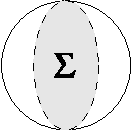
\includegraphics[width=1.2cm]{Sigma} 
\includegraphics[width=1.2cm]{g}
= 
\includegraphics[width=1.2cm]{g0}
+ 
\includegraphics[width=1.2cm]{G0SigmaHG.pdf}
\]



\end{document}
